\documentclass{beamer}
\usepackage[utf8]{inputenc}
\usepackage{listings}
\usepackage{booktabs}
\usepackage{amssymb}
\usepackage{nicefrac}
\usepackage{amsmath}
\usepackage{bbm}
\usepackage{bm}
\usepackage{enumitem}
\usepackage{hyperref}
\usepackage[export]{adjustbox}
\usepackage{svg}

\usetheme{Madrid}
\definecolor{mlpblue}{rgb}{0.1, 0.14, 0.24}

\useoutertheme{infolines} % Alternatively: miniframes, infolines, split
\useinnertheme{circles}
\usecolortheme[named=mlpblue]{structure}

\DeclareMathOperator{\Tr}{Tr}
\DeclareMathOperator{\Cov}{Cov}
\DeclareMathOperator{\Concat}{Concat}

\DeclareMathOperator*{\clip}{clip}
\DeclareMathOperator*{\argmax}{arg\,max}
\DeclareMathOperator*{\argmin}{arg\,min}
\DeclareMathOperator*{\indep}{\perp \!\!\! \perp}

\lstset{basicstyle=\footnotesize\ttfamily,breaklines=true}

%------------------------------------------------------------
%This block of code defines the information to appear in the
%Title page
\title[DeepSeek R1]{DeepSeek R1: Reasoning via RL\thanks{\href{https://raw.githubusercontent.com/deepseek-ai/DeepSeek-R1/refs/heads/main/DeepSeek_R1.pdf}{Guo, et.~al.~[Jan 2025]}}}

\subtitle{\$6M Is All You Need?}

\author[Machine Learning @ Purdue] % optional
{J.~Setpal} 

\date{January 30, 2025}

\titlegraphic{
\includegraphics[width=7cm]{../shared/logo-long.pdf}}

%End of title page configuration block
%------------------------------------------------------------

%The next block of commands puts the table of contents at the 
%beginning of each section and highlights the current section:

\AtBeginSection[]
{
  \begin{frame}
    \frametitle{Outline}
    \tableofcontents[currentsection]
  \end{frame}
}
% ------------------------------------------------------------


\begin{document}

\frame{\titlepage}

\begin{frame}{Welcome to Reading Group!}
	Ask many, many questions! \textbf{Please don't hold questions until the end.} \pause \newline \\
	Discussion is awesome, restating the obvious is good practice and boosts clarity for everyone. \pause \newline \\
	I probably get some things wrong, and definitely can't answer every question. Idea is to work through it together.
\end{frame}


%---------------------------------------------------------
% This block of code is for the table of contents after
% the title page
\begin{frame}
\frametitle{Outline}
\tableofcontents
\end{frame}
%---------------------------------------------------------

\section{RL Review}
{\let\oldfootnoterule\footnoterule
\def\footnoterule{\only<2->\oldfootnoterule}
\begin{frame}{PPO}
	We start with the standard clipped surrogate objective introduced in PPO:
	\begin{gather}
		\begin{split}
			&\mathcal{J}_{PPO}(\theta) := \mathbb{E}[q \sim P(Q), \{o_i\}^G_{i=1} \sim \pi_{\theta_{old}}(O | q)] \\
			&\frac{1}{G} \sum^G_{i=1} \min \left(\frac{\pi_{\theta_{old}}(o_i | q, o_{<i})}{\pi_\theta(o_i | q, o_{<i})} A_i, \clip \left( \frac{\pi_{\theta_{old}}(o_i | q, o_{<i})}{\pi_\theta(o_i | q, o_{<i})}, 1 \pm \varepsilon \right)  A_i \right) \\
		\end{split}
	\end{gather} \pause

	One issue with this is $A_i$, which is computed using the \textbf{Generalized Advantage Estimator}\footnote<2->{\href{https://arxiv.org/abs/1506.02438}{Schulman et.~al [ICLR 2016]}} --
	\begin{enumerate}[label=\arabic*.]
		\item Estimates long-range trajectory rewards. \pause \\
		\item However, requires a neural reward model which is expensive to train and can be unstable.
	\end{enumerate}
\end{frame}
}

\begin{frame}{RLHF Synopsis ($\nicefrac{1}{2}$)}
	We'll review the RLHF pipeline per Zeiger et al. It has 3-primary phases:
	\begin{enumerate}[label=\arabic*.]
		\item \textbf{Supervised Fine-Tuning (SFT)}: A pre-trained LLM ($\pi_{PT}$) is fine-tuned on \underline{high-quality}, domain-specific datasets to obtain $\pi_{SFT}$. \pause
		\item \textbf{Reward Modelling:} Next, we obtain a reward model $r_\phi(x,y)$ that models user preferences. \pause We start by sampling from $\pi_{SFT}$:
			\begin{gather}
				\mathcal{D} := \{(x_j, y_1, y_2)\}^{N,K}_{i=1,j=1} \sim \pi_{SFT}(y|x), \{x_i\}^K_{i=1} \\
				y_w \succ y_l | x \sim r^*(x,y)~\forall~(y_1, y_2) \in \mathcal{D}
			\end{gather}
			where $r^*(x,y)$ is the unknown optimal policy. \pause Per Bradley-Terry:
			\begin{gather}
				p^*(y_1 \succ y_2 | x) = \sigma_{softmax[y_1]}(r^*(x,y));~y \in \{y_1, y_2 \} \label{eq:3}
			\end{gather}
			is the preference distribution optimized over \underline{negative log-likelihood} on a parameterized model $r_\phi(x,y)$. \pause Some notes:
			\begin{enumerate}[label=\alph*.]
				\item Rewards are normalized over $x$ to motivate lower variance. \pause
				\item $r_\phi$ is $\pi_{SFT}$ with the final linear layer returning the scalar reward.
			\end{enumerate}
	\end{enumerate}
\end{frame}

\begin{frame}{RLHF Synopsis ($\nicefrac{2}{2}$)}
	\begin{enumerate}
		\item[3.] \textbf{RL Fine-Tuning:} Finally, we use $r_\phi$ to fine-tune $\pi_{SFT}$, with the following objectives:
			\begin{enumerate}[label=\alph*.]
				\item $r_\phi$ should be maximized. \textbf{Assumption:} $r^* \approx r_\phi$. \pause
				\item We \textit{do not} want mode-collapse (random tokens that maximize reward). \pause \textbf{Solution:} \underline{KL Divergence}. \pause
			\end{enumerate}
			Mathematically, RLHF posits the following optimization problem:
			\begin{gather}
				\max_{\pi_\theta}\mathbb{E}_{x\sim\mathcal{D}, y \sim \pi_\theta(y|x)}(r_\phi(x,y)) -\beta \mathbb{D}_{KL}[\pi_\theta(y|x)~||~\pi_{SFT}(y|x)]
			\end{gather} \pause
			This is equivalent to the reward function:
			\begin{gather}
				r(x,y) = r_\phi(x,y) - \beta(\log \pi_\theta(y|x)) - \log(\pi_{SFT}(y|x))
			\end{gather}
			Which is maximized using \textbf{Proximal Policy Optimization}.
	\end{enumerate}
\end{frame}

\begin{frame}{GRPO ($\nicefrac{1}{2}$)}
	For each question $q$, GRPO samples outputs $\{o_1, \ldots, o_G\}$ with the training objective being to maximize (1):
	\begin{gather}
		\begin{split}
			&\mathcal{J}_{GRPO}(\theta) := \mathbb{E}[q \sim P(Q), \{o_i\}^G_{i=1} \sim \pi_{\theta_{old}}(O | q)] \\
			&\frac{1}{G} \sum^G_{i=1} \left(\min \left(\frac{\pi_{\theta_{old}}(o_i | q)}{\pi_\theta(o_i | q)} A_i, \clip \left( \frac{\pi_{\theta_{old}}(o_i | q)}{\pi_\theta(o_i | q)}, 1 \pm \varepsilon \right)  A_i \right) + \beta D_{KL}(\pi_\theta || \pi_{\text{ref}}) \right) \\
		\end{split} \\
		D_{KL}(\pi_\theta || \pi_{\text{ref}}) = \frac{\pi_{\text{ref}}(o_i | q)}{\pi_\theta(o_i | q)} - \log \frac{\pi_{\text{ref}}(o_i | q)}{\pi_\theta(o_i | q)} - 1 \\
		A_i = \frac{r_i - \bar{r}}{\sigma_{std}(r)};\ r \in \{r_1, \ldots, r_G \}
	\end{gather}
\end{frame}

\begin{frame}{GRPO ($\nicefrac{2}{2}$)}
	We have defined everything except the reward function. \pause Unfortunately the paper also is vague about this\pause; it specifies a \underline{rule-based} system:
	\begin{enumerate}[label=\arabic*.]
		\item \textbf{Accuracy rewards:} For objective tasks, correctness $\propto$ reward .\pause
		\item \textbf{Format rewards:} For following the required format, it gets a reward. \pause
	\end{enumerate}

	\begin{center}
		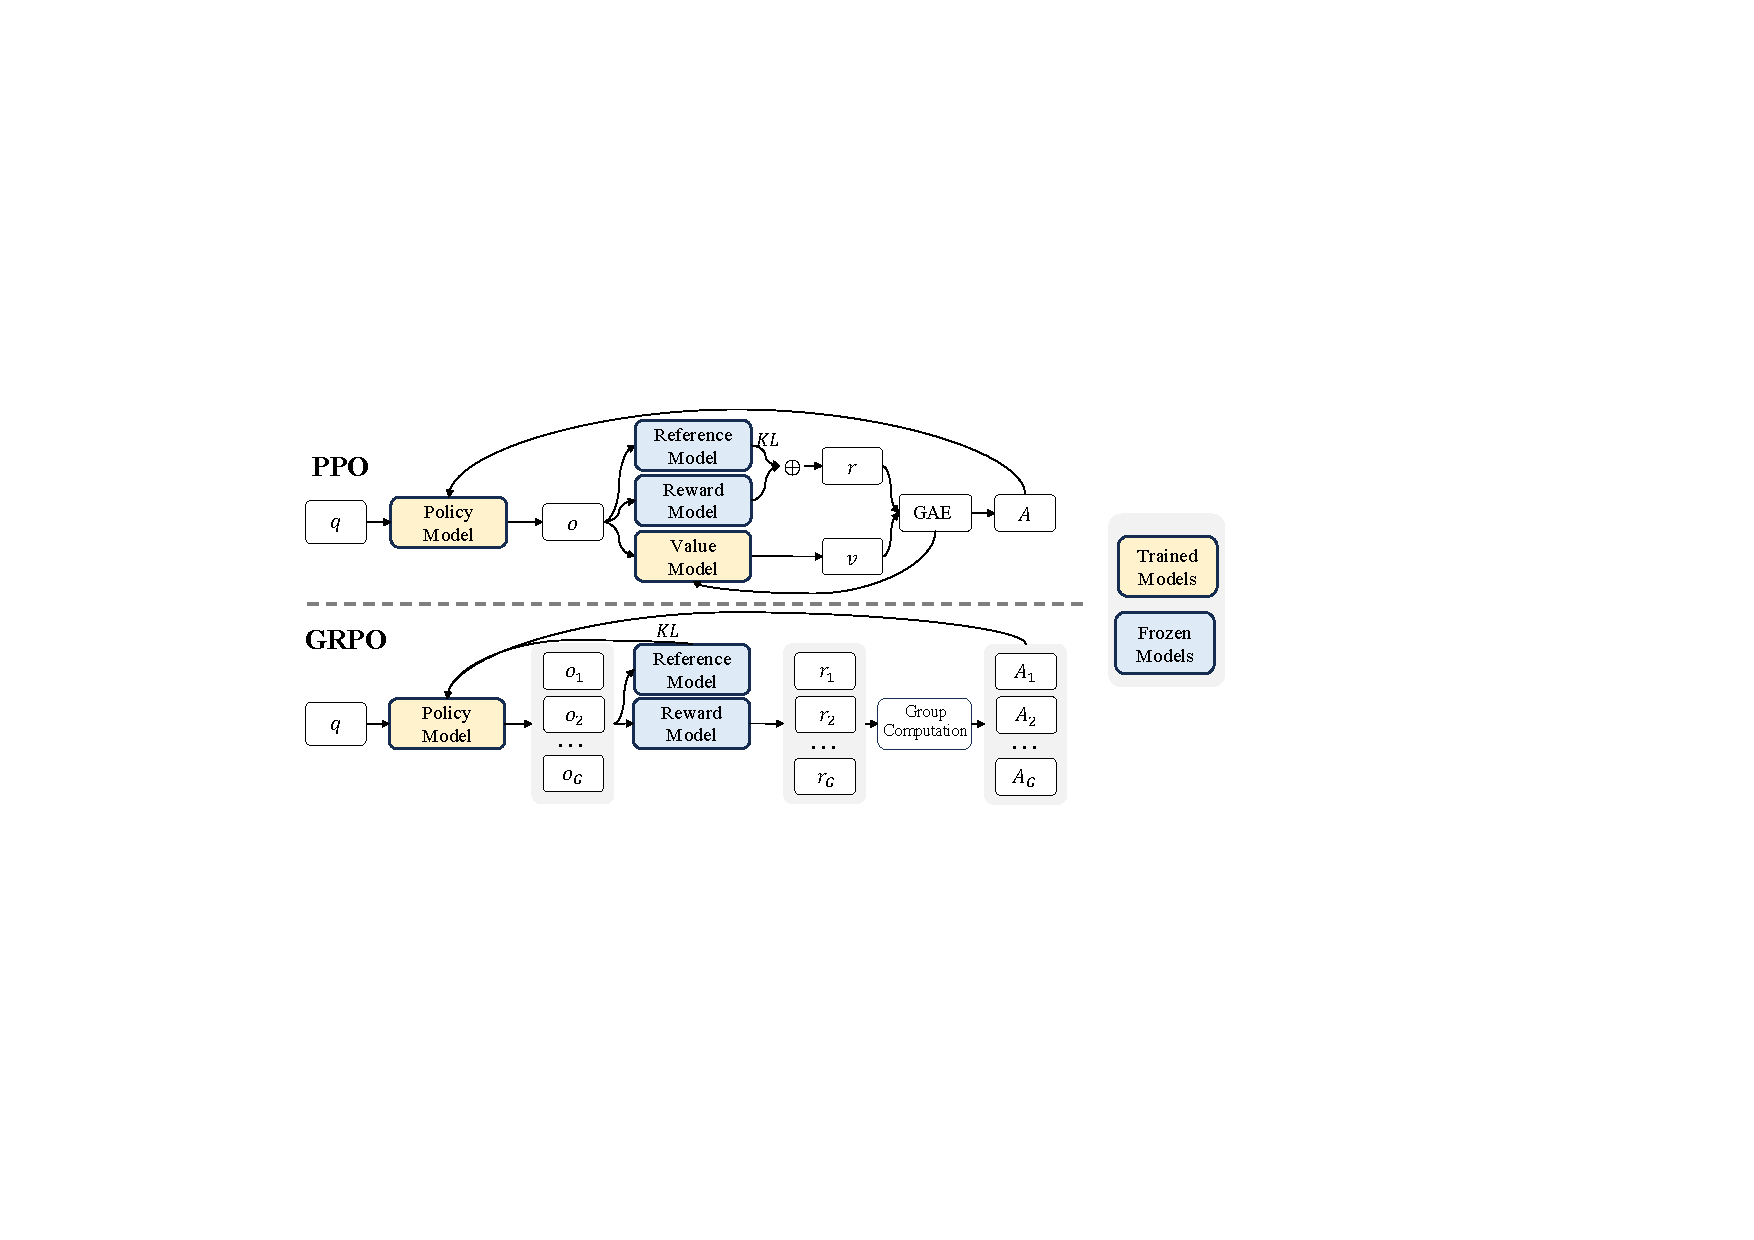
\includegraphics[width=\textwidth]{img/GRPO.pdf}
	\end{center}
\end{frame}

\section{Training Details}
\begin{frame}{Approach Overview}
	The training process can largely can be broken down into three stages:
	\begin{enumerate}[label=\arabic*.]
		\item \textbf{RL on a base model} -- gets us DeepSeek-R1-Zero.
		\item \textbf{RL+SFT on a checkpoint} -- gets us DeepSeek-R1.
		\item \textbf{Distillation} -- gets us DeepSeek-R1-Distill-\texttt{<model-name>}.
	\end{enumerate}
	~ \\

	We'll discuss each of these in detail next.
\end{frame}

\begin{frame}{Less is More Philosophy}
	A core finding from \underline{Less is More for Aligment (LIMA)}\footnote{\url{https://arxiv.org/abs/2305.11206}} -- a small set of \textit{synethetic} examples encourages better generalization. \pause \newline \\

	\textit{Less} (controlled) randomness, unbiased initialization in unstable regimes can avoid local optima and training failures. \pause \newline \\

	This is strong exemplified in the approaches used for R1's training: \pause
	\begin{enumerate}[label=\arabic*.]
		\item \textit{No need} for neural rewards, don't want reward hacking. \pause \\
		\item \textit{No need} for SFT, let GRPO figure it out from scratch. \pause \\
		\item \textit{No need} for complex prompting, don't bias RL towards approaches. \pause \\
	\end{enumerate}
	~ \\
	This, combined with \textbf{carefully selected data} are key to the incredible benchmark performance.
\end{frame}

\begin{frame}{RL on a Base Model}
	Start by taking a base model (no SFT, but models language well). \pause \newline \\

	Train with RL until convergence on task. \pause \textbf{Interesting consequence:}
	\begin{center}
		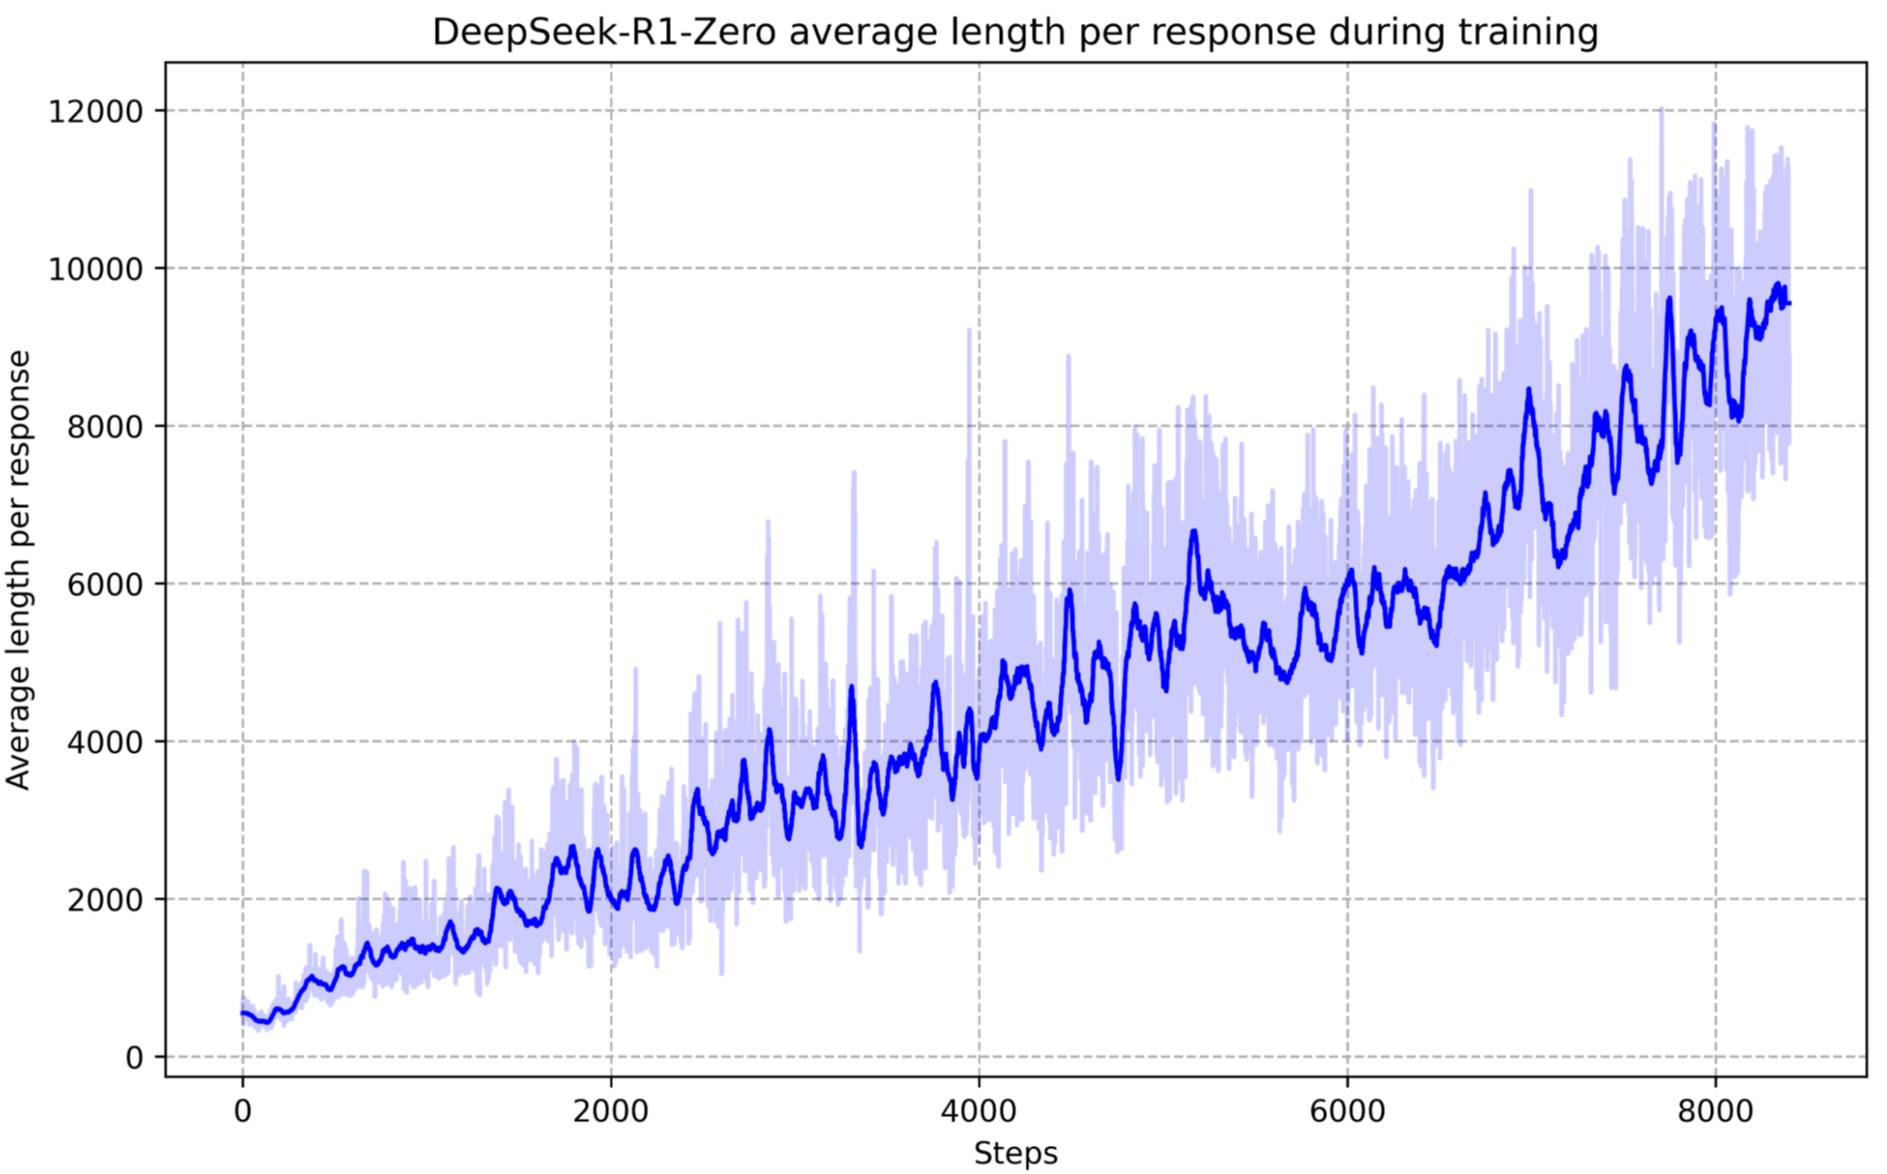
\includegraphics[width=.7\textwidth]{img/resp_len.png}
	\end{center} \pause
	\vspace{-1em}
	Thinking more, and thinking anthropomorhically as emergent properties.
\end{frame}

\begin{frame}{Challenges with Direct RL}
	There are a couple of negative consequences:
	\begin{enumerate}[label=\arabic*.]
		\item \textbf{Poor Readibility:} No rewards motivating readibility. \pause
		\item \textbf{Language Mixing:} No rewards motivating consistency of language -- although this one should have been fairly easy to implement? \pause
			\begin{block}{\bf Aside}
				They did figure this out for R1, but it degraded performance slightly.
			\end{block} \pause
	\end{enumerate}
	~ \\
	Solution? \textbf{Cold Start}. Use SFT \textit{briefly}, to encourage approaching problems consistently.
\end{frame}

\begin{frame}{Cold Start}
	So, what is cold start? \\
	\textbf{Idea:} Collect small amount of long CoT data; to fine-tune the base model as the initial actor. \pause \newline \\

	From here, we expect the local optima to find a solution that leverages readibility but \textit{prevents} language mixing. \pause \newline \\

	How to actually \underline{collect the data}? \pause They used a couple of strategies:
	\begin{enumerate}[label=\arabic*.]
		\item Few shot prompting using a long CoT as examples. \pause \\
		\item Prompting for detailed explanations, with reflection \& verification. \pause \\
		\item Manually refining DeepSeek-R1-Zero outputs to remove language mixing, fixing readibility and general response refinment.
	\end{enumerate}
\end{frame}

\begin{frame}{Rejection Sampling \& Supervised Fine-Tuning}
	When RL converges, use the training checkpoint to sample data from domains beyond just reasoning: creative writing, role-playing, general purpose tasks. \pause \newline \\

	\textbf{Beyond Rule-Based Rewards Modelling:} 
	\begin{enumerate}[label=\arabic*.]
		\item Curate reasoning prompts and rejection sampling from the checkpoint. \pause
		\item Now, incorporate generative reward model -- DeepSeek-V3. \pause
		\item Sample multiple responses and retain correct ones.
	\end{enumerate}
	Overall, we get from this $\approx 600$K reasoning related training samples. \pause \newline \\

	Next, add $\approx 200$K tokens for factual QA, self-cognition, translation, etc. \pause \newline \\

	Add CoT where relevant, using DeepSeek-V3. \pause \newline \\

	SFT DeepSeek-V3-Base for 2 epochs over $\approx 800$K sample dataset. \pause \textbf{Profit}.
\end{frame}

\begin{frame}{Secondary RL Stage}
	This part is \textit{exactly} RLHF. \pause \newline \\

	Helps with: improving helpfulness and harmlessness. \pause
	\begin{block}{Quiet Part Out Loud}
		Probably was used to filter out Tiananmen Square Massacre information, whatever additional censorship they desire.
	\end{block}
\end{frame}

\begin{frame}{Distillation}
	Further, they fine-tuned open source models like Qwen \& LLaMa over DeepSeek-R1's responses. \pause \newline \\

	Here, used SFT and not RL even though they think RL would peform better. \pause \newline \\

	\begin{block}{\bf Opinion}
		I disagree, they could've used RL to fine-tune DeepSeek-V3-Base with RL-checkpointed data but chose SFT.
	\end{block}

\end{frame}

{\let\oldfootnoterule\footnoterule
\def\footnoterule{\only<3->\oldfootnoterule}
\begin{frame}{What \underline{Didn't} Work \& Why}
	\textbf{Process Reward Model}: Prone to reward hacking, requires fine-grained setup, evaluating intermediate steps are challenging for general reasoning. \pause \newline \\

	\textbf{Monte-Carlo Tree Search}: Enable explore the solution space systematically; however here search space is ill-degined and very restrictive. \pause \newline \\
	Setting restrictions leads to spurious local optima, and also requires a pre-trained value model which is expensive. \pause \newline \\

	\begin{block}{Aside}
		Approaches do exist that combine these two and exhibit strong performance in specific specialized domains.\footnote<3->{\url{https://arxiv.org/abs/2406.03816}}\footnote<3->{\url{https://arxiv.org/abs/2501.07301}}
	\end{block}
\end{frame}
}

\begin{frame}{Drawbacks}
	The authors note the following limitations of their approach:
	\begin{enumerate}[label=\arabic*.]
		\item Their reasoning focused approach triggers some catastrophic forgetting. \pause \\
		\item It reasons in English / Chinese even when query language is neither. \pause \\
		\item It doesn't work well with few-shot prompting. \pause \\
		\item It doesn't work well for SWE tasks.
	\end{enumerate}
\end{frame}

\section{Performance Evals}

\begin{frame}{Reasoning}
	\begin{center}
		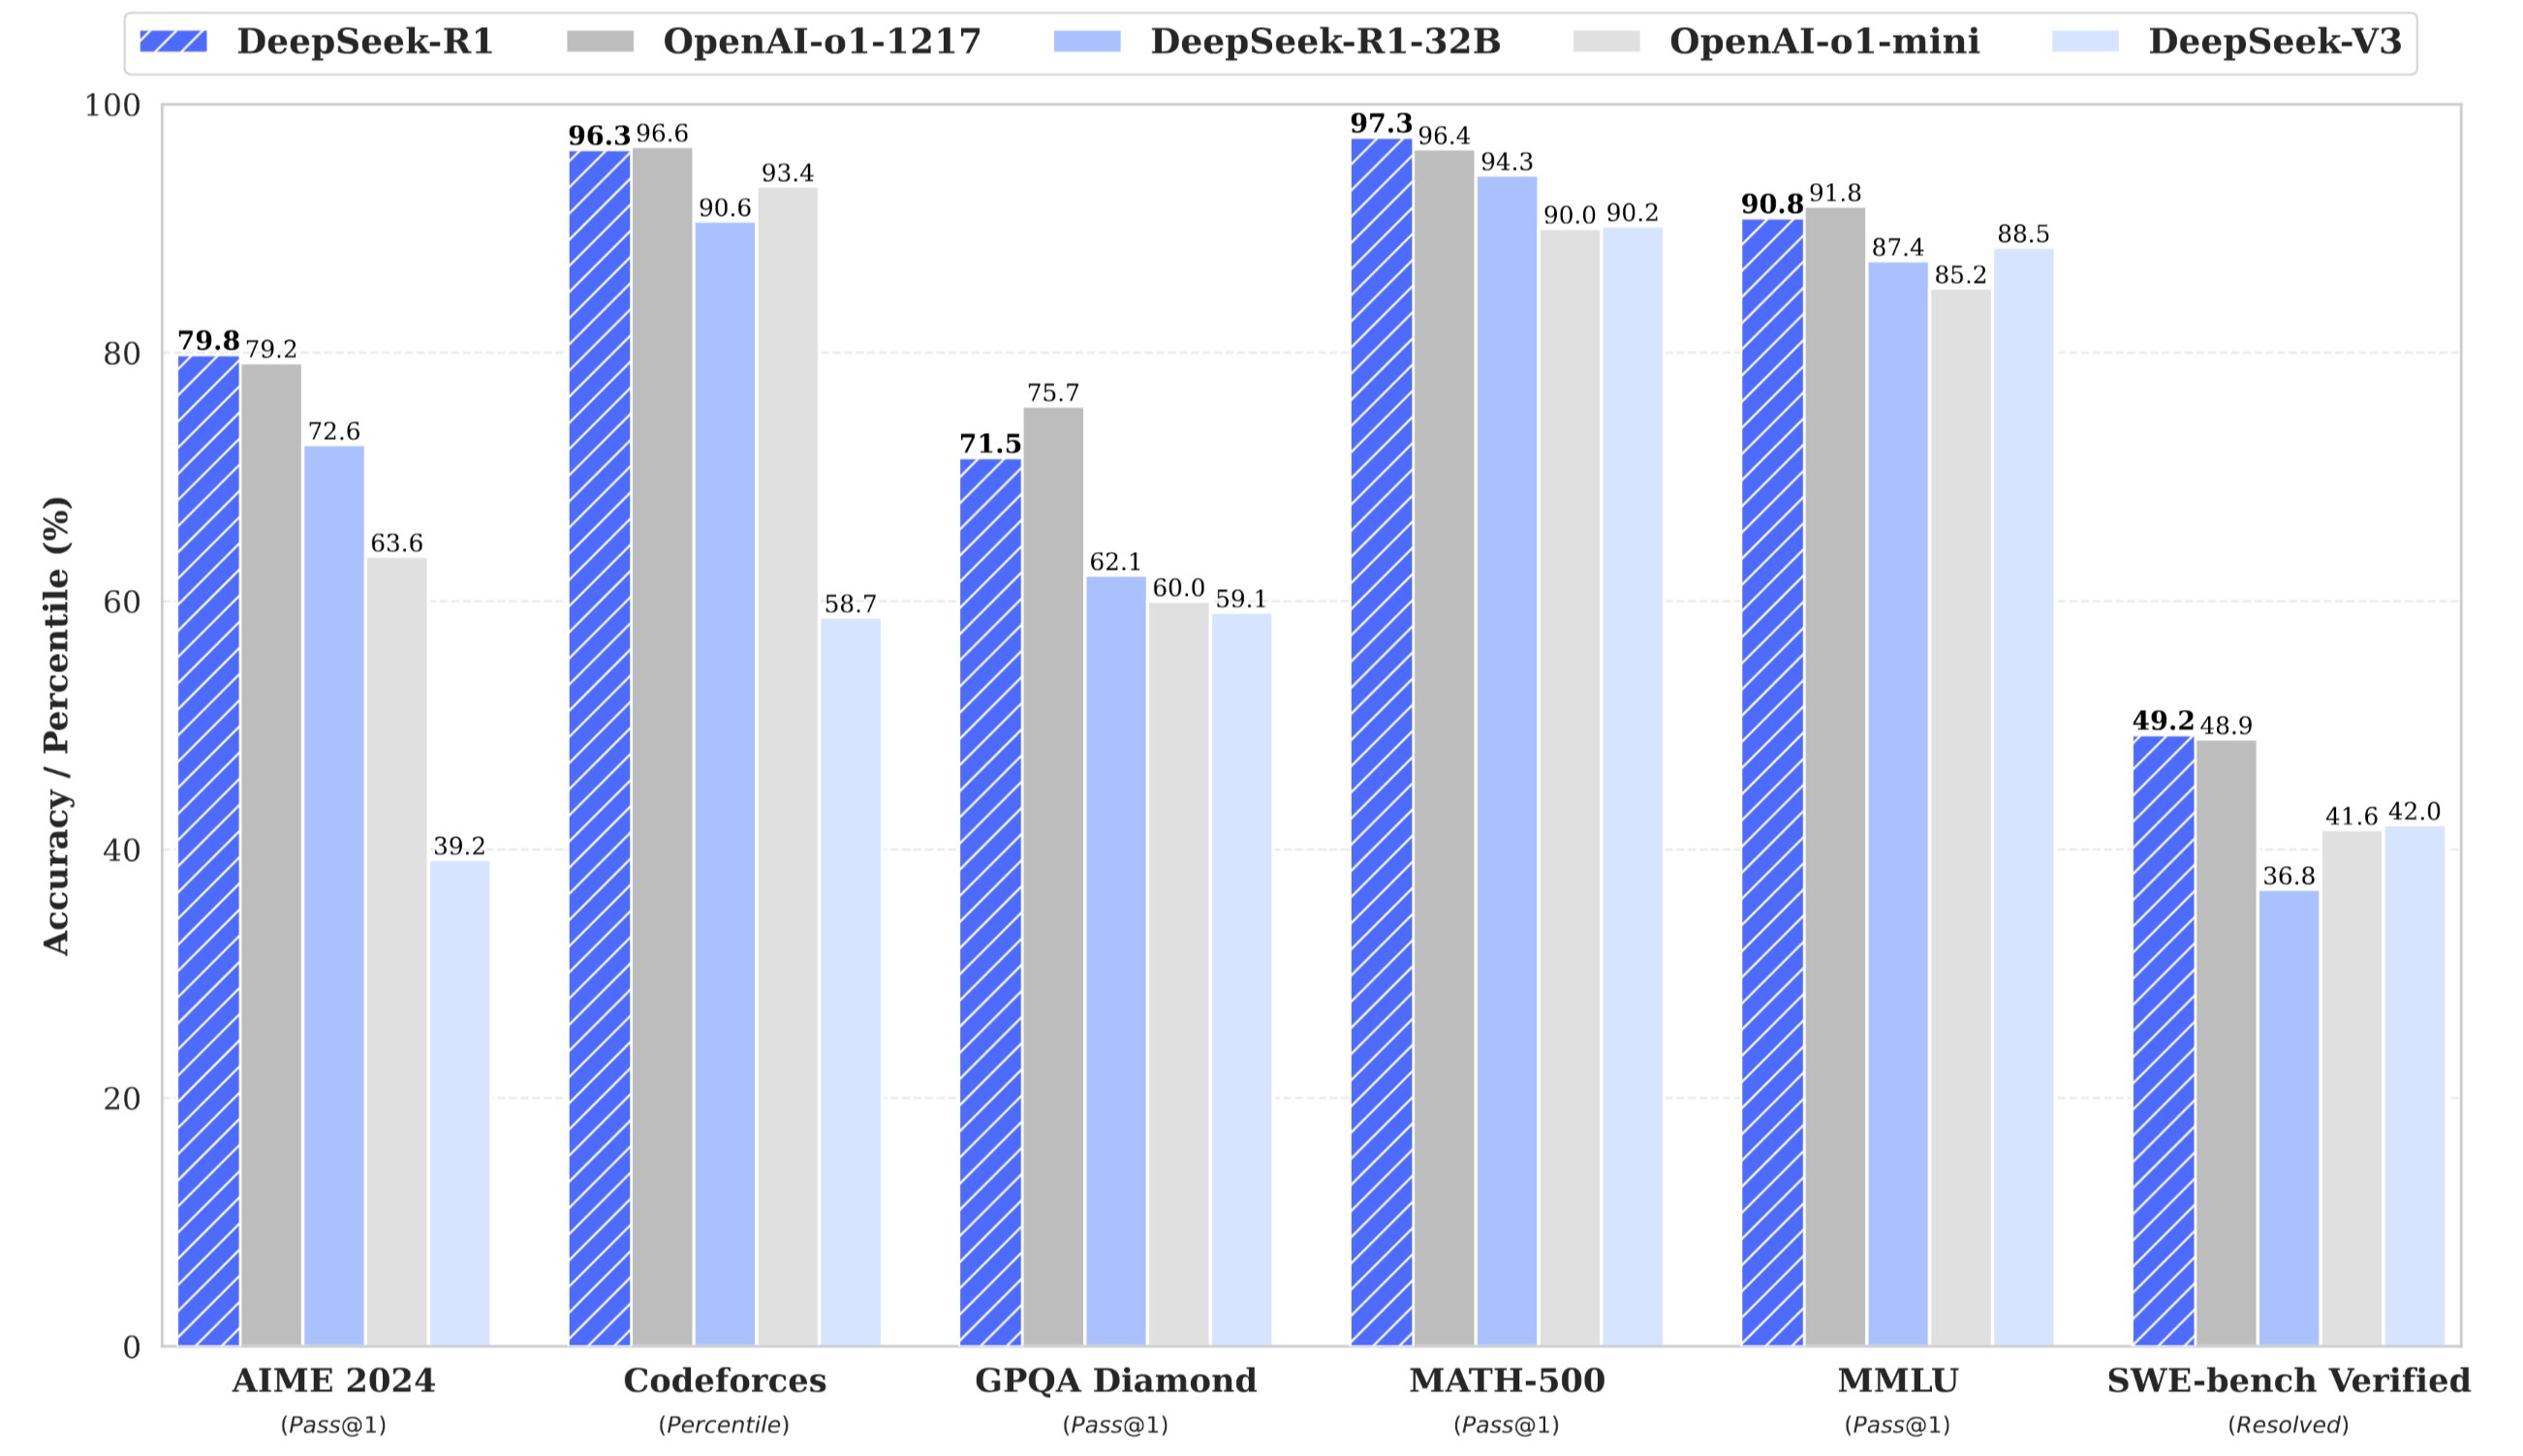
\includegraphics[width=\textwidth]{img/benchmarks.png}
	\end{center}
\end{frame}

\begin{frame}{Other Stuff}
	\begin{center}
		[Refer to paper directly]
	\end{center}
\end{frame}

\begin{frame}{Thank you!}
	\begin{center}
		Have an awesome rest of your day!
	\end{center}
	\begin{center}
		\textbf{Slides:} \url{https://jinen.setpal.net/slides/dsr1.pdf}
	\end{center}
\end{frame}

\end{document}
